\chapter{Introduction}
Avant l'introduction de ResNet en 2015 par \citeauthor{resnet}, l'architecture GoogLeNet était le dernier gagnant des challenges de vision par ordinateur. Cette architecture avait été développée pour pallier les problèmes d'apprentissage liés à l'augmentation de la profondeur de VGG, une autre architecture proéminente.

Un réseau plus profond peut offrir de meilleures performances dans certaines conditions, mais il est aussi sujet à des problèmes tels que l'explosion ou l'évanouissement du gradient de la fonction de coût. Durant la rétropropagation, les grandes ou petites valeurs de gradient peuvent s'amplifier à travers les couches du réseau, entraînant un gradient bien plus grand ou plus petit dans les dernières couches par rapport aux premières. Cet effet est multiplicatif et dépend donc de la profondeur du réseau.

Pour un réseau d'une profondeur $L$, on modélise ces états cachés de chaque couche de dimension $d$ par une séquence $(h_k)_{1 \leq k \leq L}$ avec $h_k \in \mathbb{R}^d, \forall 0 \leq k \leq L$. L'explosion du gradient peut être décrite mathématiquement par, avec une forte probabilité, $\| \frac{\partial \mathscr{L}}{\partial h_0} \| \gg \| \frac{\partial \mathscr{L}}{\partial h_L} \|$, où $\mathscr{L}$ représente la loss et $\left\| \cdot \right\|$ la norme euclidienne.

GoogLeNet, bien qu'offrant une légère amélioration des performances par rapport à VGG, était encore relativement complexe et sa profondeur comparable à celle de VGG, passant de 22 à 16 couches. En 2015, Microsoft introduit ResNet, un modèle allant jusqu'à 152 couches et divisant par deux le nombre d'erreurs de GoogLeNet. Son innovation réside dans l'intégration de \textit{skip connections} entre les couches successives, facilitant le passage du gradient au sein du réseau. Mathématiquement, cela donne la relation récurrente suivante pour la séquence $(h_k)_{1 \leq k \leq L}$ :
\[
    h_{k+1} = h_k + f(h_k, \theta_{k+1})
.\]

où $f(\cdot, \theta_{k+1})$ représente les transformations effectuées par la couche $k$ et paramétrées par $\theta_{k+1} \in \mathbb{R}^p$.

Les ResNets sont devenus la base de nombreux modèles d'apprentissage profond de pointe, s'étendant au-delà du traitement d'images pour inclure des domaines tels que le traitement du langage naturel et l'apprentissage par renforcement. L'idée des \textit{skip connections} a inspiré de nombreuses autres architectures et est devenue une pratique courante dans la conception des réseaux neuronaux profonds.

\begin{figure}[H]
    \centering
    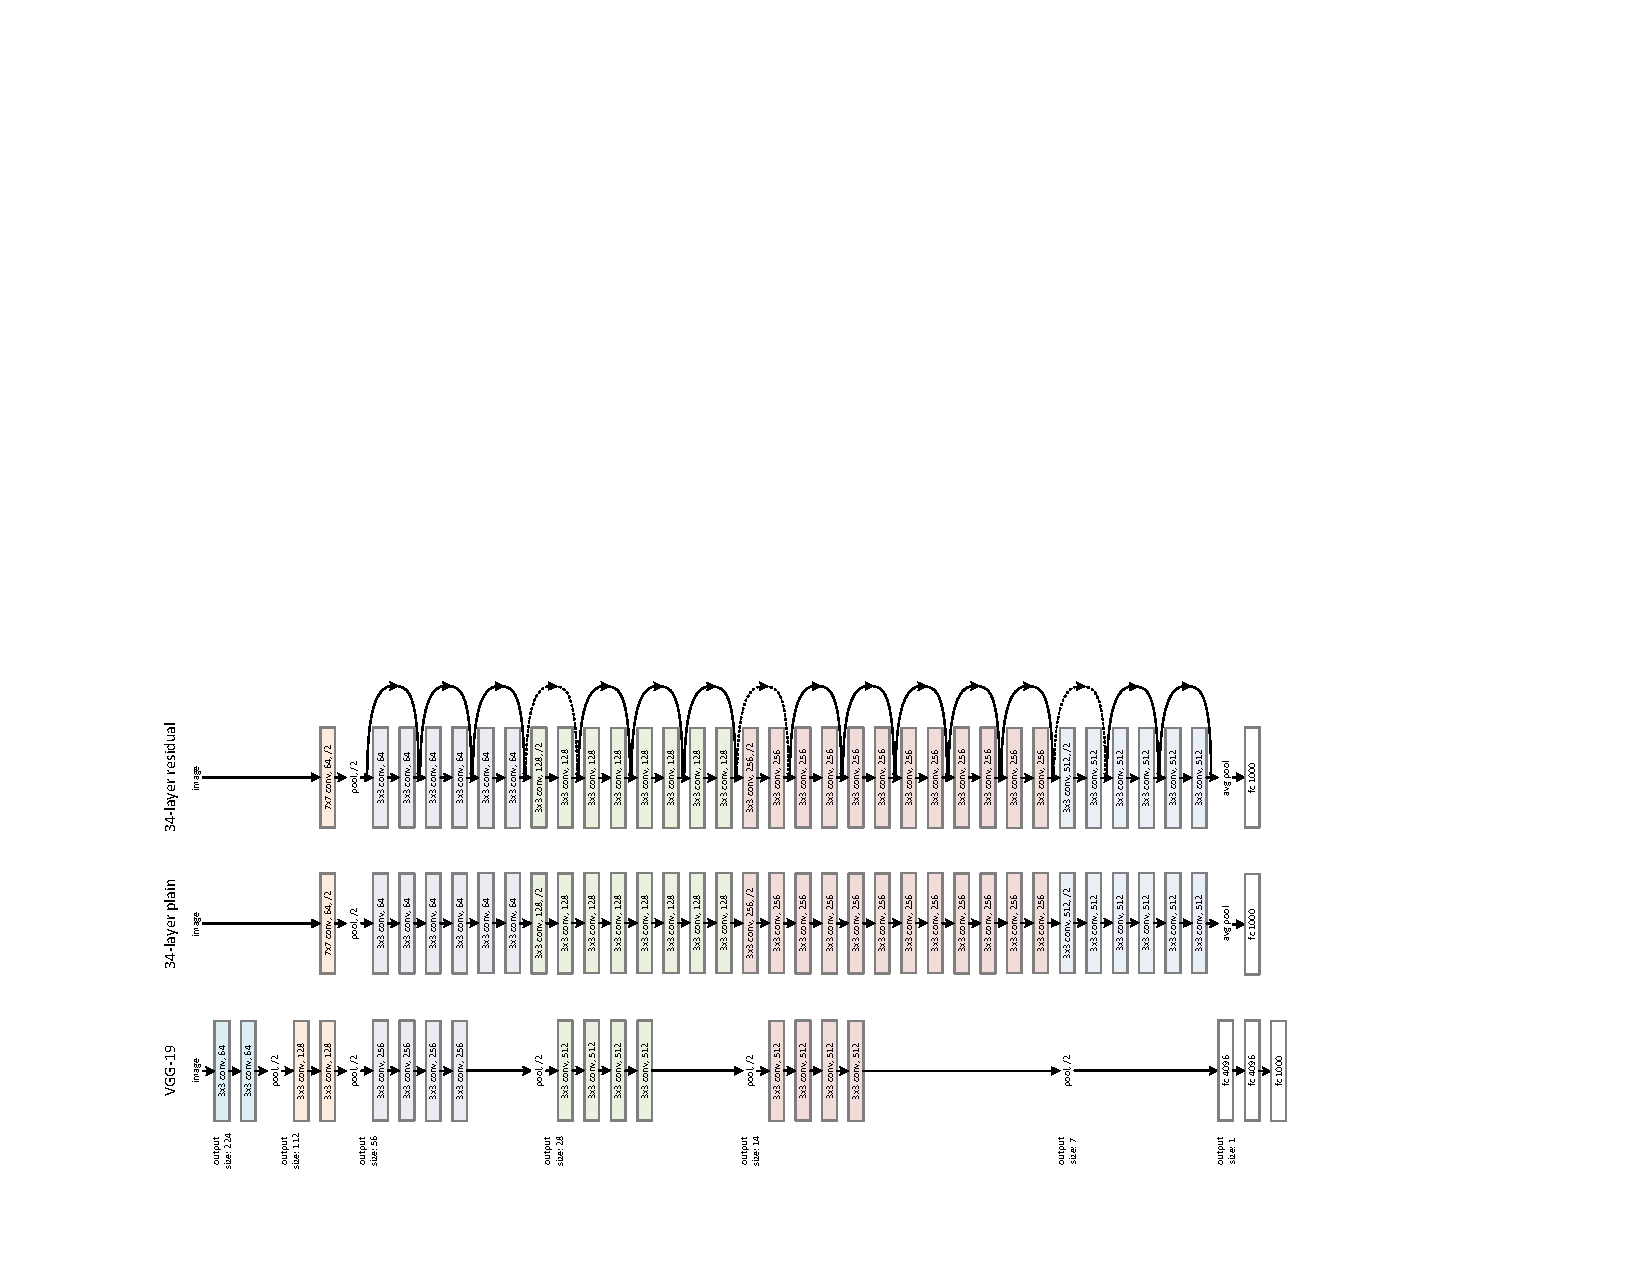
\includegraphics[width=.9\textwidth]{figs/resnet_arch.pdf}
    \caption{Example d'architecture pour la vision par ordinateur. \textbf{Bas} : VGG-19 (19.6 billion FLOPs). \textbf{Millieu} : un réseau classique (3.6 billion FLOPs). \textbf{Haut} : Un réseau résiduel (3.6 billion FLOPs) avec la présence de \textit{skip connections} dans chaque bloc. Figure extraite de l'article original de ResNet \citep{resnet}}
    \label{fig:resnet}
\end{figure}

Malgré ces avancées, ResNet rencontre toujours des problèmes de gradient durant l'apprentissage. La méthode traditionnelle pour contrer cela est la normalisation des états cachés après chaque couche (\textit{batch normalization}). Cependant, cette approche a un coût computationnel et dépend fortement de la taille du \textit{batch}. Une alternative est d'incorporer un facteur d'échelle $\alpha_L$ devant le terme résiduel, conduisant au modèle suivant :
\begin{equation}\label{resnet_equation}
    h_{k+1} = h_k + \alpha_L f(h_k, \theta_{k+1})
\end{equation}
Le choix de $\alpha_L$ est crucial et dépend naturellement de la profondeur $L$ du réseau. Il assure que la variance du signal reste stable lors de sa propagation à travers les couches. Cependant, il n'existe actuellement ni preuve formelle ni justification mathématique solide pour le choix de ce facteur de régularisation.

Dans ce cours, nous examinerons les fondements mathématiques pour choisir la valeur de $\alpha_L$ en fonction de $L$ et de la distribution initiale des poids, dans le but d'éviter les problèmes d'apprentissage. Deux axes principaux d'étude seront abordés :
\begin{enumerate}
    \item Le facteur $\alpha_L$ à l'initialisation : L'initialisation des paramètres est cruciale pour la phase d'apprentissage d'un modèle et influe même sur ses capacités de généralisation. Une mauvaise initialisation peut entraîner une divergence ou une disparition rapide du gradient, voire un blocage dans l'apprentissage. L'étude du rôle de $\alpha_L$ lors de l'initialisation est donc pertinente. Nous considérerons que, à l'initialisation, les poids de chaque couche $(\theta_k)_{1 \leq k \leq L}$ sont choisis de manière indépendante et identique selon une loi, typiquement gaussienne ou uniforme sur $\mathbb{R}^p$. 
    % \item L'approche continue : Bien que le réseau neuronal soit constitué de nombreuses couches distinctes, l'ensemble du réseau peut être considéré comme une fonction, lorsqu'il y a suffisament de neurones. L'idée centrale des équations différentielles neuronales est de traiter les couches distincts du réseau comme continues, en supposant que chaque couche subit de petits changements. Ainsi, l'entrée de la couche suivante est considérée comme le résultat de l'intégrale de l'entrée de la couche précédente. Cela peut être comparé au mouvement d'un projet, où le déplacement dans la deuxième seconde peut être approximé par la déplacement dans la première seconde plus la vitesse dans la première seconde (multipliée par l'intervalle de temps d'une seconde).
    % Les équations différentielles neuronales ont ouvert une nouvelle direction pour la théorie et la pratique de l’apprentissage profond et ont été appliquées à la classification d’images, aux séries chronologiques et à d’autres domaines. Tous les réseaux d'apprentissage profond avec des connexions résiduelles peuvent être exprimés approximativement par des équations différentielles neuronales
    \item L'approche continue : Dans les réseaux neuronaux composés de nombreuses couches, l'ensemble peut être considéré comme une fonction continue, particulièrement lorsque le nombre de neurones est élevé. Cette méthode envisage le réseau non pas comme une série de couches discrètes, mais plutôt comme un système continu. En adoptant cette vue, chaque couche est perçue comme une évolution marginale de la précédente, similaire à l'idée derrière les connexions résiduelles de ResNet. On peut imaginer que l'entrée de chaque couche suivante résulte de l'intégration des ajustements minimes apportés par la couche précédente, une approche semblable à la modélisation du mouvement en physique, où la position est intégrée sur le temps.\\
    Les EDN représentent une avancée significative dans la théorie et la pratique de l'apprentissage profond, trouvant des applications dans la classification d'images, l'analyse de séries temporelles et d'autres domaines. Il est intéressant de noter que tout réseau de deep learning doté de connexions résiduelles peut être approximativement exprimé par des équations différentielles neuronales.
\end{enumerate}